%%%% ijcai11.tex

\typeout{Paper over muisbesturing a.d.h.v EOG}

\documentclass{article}
\usepackage{ijcai11}
\usepackage[dutch]{babel}
\usepackage[utf8]{inputenc}

% Use the postscript times font!
\usepackage{times}
\usepackage{float}
\usepackage{hhline}
\usepackage[pdftex]{graphicx} 
\usepackage{caption}
\usepackage{amsmath}
\usepackage{fancyhdr}
\usepackage{wrapfig}
\usepackage{url}

\newcommand{\figwidth}{0.82\linewidth}

\title{Muisbesturing aan de hand van Elektro-Oculografie.}
\author{Pieter Verlinden \& Michiel Willems}

%Plot packages
\usepackage{siunitx}
\usepackage{tikz} % To generate the plot from csv
\usepackage{pgfplots}

\pgfplotsset{compat=newest} % Allows to place the legend below plot
\usepackage{pgfplotstable}
\usetikzlibrary{arrows,shapes,positioning,fit,shapes.misc,matrix,decorations.text,shapes.geometric}
\usepgfplotslibrary{units} % Allows to enter the units nicely

\sisetup{
	round-mode          = places,
	round-precision     = 2,
}
% -----------------------------------

\pagestyle{plain}

\begin{document}



\maketitle

\begin{abstract}
  Gebruikmakende van apparatuur voor elektro-oculografie, ontwikkeld door het Innovation Lab aan de KULeuven, worden er mechanismen aangeboden die een muisaanwijzer kan besturen aan de hand van toestanden. Deze mechanismen kunnen op hun beurt apart onderzocht worden en geoptimaliseerd worden. Typische problemen die optreden bij elektro-oculografie en specifieke eigenschappen van de apparatuur van het Innovation Lab, worden onderzocht en aangepakt door de voorgestelde mechanismen.
\end{abstract}

\section{Inleiding}
In deze paper worden de resultaten en bevindingen van onderzoek naar signaal interpretatie, met muisbesturing als doel, getoond en besproken. Eerst zal het doel van het onderzoek aan bod komen. Daarna zal er een technische achtergrond geschetst worden over elektro-oculografie en  de gebruikte apparatuur en wordt er een korte motivatie gegeven waarom onderzoek en ontwikkeling in deze technologie belangrijk is. Verder komt de probleemstelling van het onderzoek aan bod waarin de problemen worden besproken die ondervonden werden tijdens het onderzoek. In de daarop volgende sectie wordt er getracht om oplossingen voor deze problemen aan te bieden.\\
Tot slot worden de testparameters en de experimenten besproken met de resultaten en een conclusie als finaal besluit van deze paper. 
\subsection{Doel}
Het doel van het onderzoek is om te kijken in hoeverre het mogelijk is om signalen, verkregen via elektro-oculografie, te interpreteren en te gebruiken om een computermuis aan te sturen. Bijkomstig is de nauwkeurigheid hiervan verbeteren naarmate de gebruiker het programma langer gebruikt en een mogelijkheid bieden om het voor elke gebruiker toegankelijk te maken met bijvoorbeeld de hulp van training applicaties. 

\subsection{EOG technologie}
Elektro-oculografie is een techniek waarbij men het biopotentiaal tussen de voorkant en de achterkant van het menselijk oog tracht  op te meten.  Het oog gedraagt zich als een dipool (figuur \ref{fig:oogdipool}) waarbij de voorkant positief geladen is en de achterkant negatief \cite{yagi:eoginterface}. Wat belangrijk is in de context van het vastleggen van oogbewegingen, is dat dit biopotentiaal verandert naarmate er in verschillende richtingen gekeken wordt. Deze signaalvariatie is duidelijk meetbaar in het geval van beduidende ooghoekvariaties, wat het mogelijk maakt om duidelijk onderscheid te maken tussen vooraf bepaalde oogbewegingen (in het geval van dit onderzoek: links, rechts, boven en onder).
\begin{figure}[H]
	\centering
	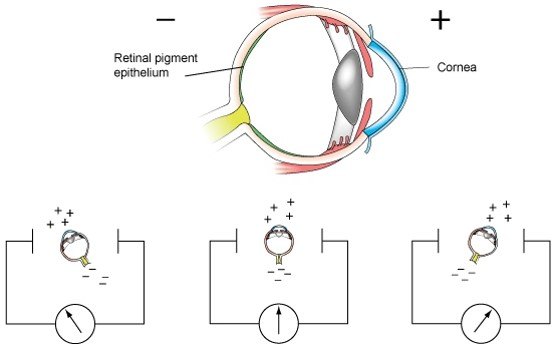
\includegraphics[width=0.8\linewidth]{images/oogdipool}
	\caption{Illustratie van het biopotentiaal tussen het hoornvlies($+$) en netvlies($-$).}
	\label{fig:oogdipool}
\end{figure}
\begin{wrapfigure}{r}{0.40\linewidth}
	\begin{center}
		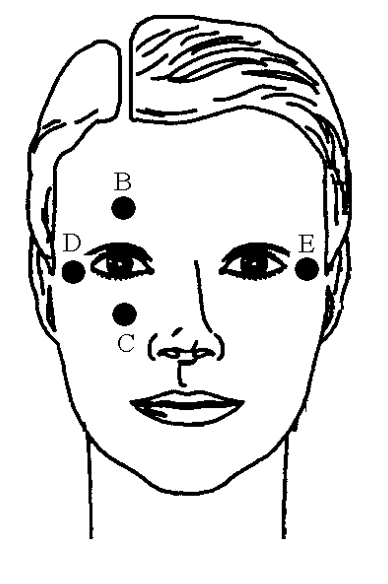
\includegraphics[width=0.1\textwidth]{images/sensorplaatsing}
		\caption{Plaatsing van de sensoren op het hoofd.}
		\label{fig:sensorplaatsing}
	\end{center}
\end{wrapfigure}
Dit biopotentiaal wordt gemeten aan de hand van vier sensoren die op het hoofd van de testpersoon worden aangebracht. Twee sensoren worden op de linker en rechter slaap van de testpersoon aangebracht, deze sensoren meten de horizontale dimensie van de gemeten oogbeweging. Twee sensoren worden boven en onder een van de ogen aangebracht, deze meten de verticale dimensie van de gemeten oogbeweging (figuur \ref{fig:sensorplaatsing}).\\

Om de signalen te kunnen meten, wordt er gebruik gemaakt een elektronische schakeling, ontwikkeld door InnovationLab KULeuven. Deze schakeling zal het signaal eerst versterken naar een waarde tussen 0 en 5$V$. Daarna wordt dit potentiaal omgezet naar een 10bit getal (dus een getal tussen 0 en 1023). Dit nu digitale signaal kan via een USB-verbinding aangesloten worden op een computer, waar het verder in detail onderzocht en gebruikt kan worden om, in dit geval een applicatie te schrijven om een muiscursor aan te sturen.

\subsubsection*{Motivatie voor de technologie}
De apparatuur om het biopotentiaal te meten is relatief goedkoop en makkelijk te produceren. Het enige wat nodig is, is een kleine printplaat waarop de componenten worden aangebracht, een USB-verbinding naar de computer en sensoren voor het hoofd.\\
Een bijkomstig voordeel is dat de sensoren makkelijk te bevestigen zijn op het hoofd, ten opzichte van andere technologie\"en die soms implantaten of de immobiliteit van het hoofd vereisen. E\'en van de grootste voordelen is dat de sensoren, wanneer goed aangebracht, het zicht weinig of niet blokkeren en niet lastig zijn voor de gebruiker.

\subsection{Algemene aanpak en terminologie}
De data die via het apparaat binnenkomt, is opgesplitst in twee signalen: een signaal voor verticale oogbewegingen (hetgeen \textit{Y-sginaal} zal genoemd worden) en een signaal voor horizontale oogbewegingen (hetgeen \textit{X-signaal} zal genoemd worden). Deze signalen worden elk verdeeld in drie toestanden. In het geval van de horizontale beweging is dit \textit{LINKS, MIDDEN, RECHTS} en in het geval van de verticale beweging is dit \textit{ONDER, MIDDEN, BOVEN}. Om deze toestanden te bepalen, wordt er gebruik gemaakt van grenswaarden of \textit{thresholds}. Bij een oogbeweging kan er een verschil in signaal berekent worden. Als dit verschil boven \'e\'en van deze grenswaarden ligt, kan er vastgesteld worden dat de toestand (mogelijk) veranderd is.
\section{Probleemstelling}
De signalen verkregen via elektro-oculografie zijn relatief eenvoudig te interpreteren maar bieden weinig nauwkeurigheid. Uitgaande van een perfect signaal zouden gemakkelijk acht richtingen (van de ogen) herkent kunnen worden m.n. de acht windrichtingen. Echter, problemen zoals ruis, het knipperen van het oog en andere problemen die verder in deze sectie besproken zullen worden, laten het voorlopig (in het programma van dit onderzoek) enkel toe om vier richtingen te herkennen. 
\subsection{Ruis}
Een eerste probleem dat optreedt is ruis. Ruis is te wijten aan een verschil in temperatuur, vochtigheid of aan bewegingen van het hoofd. Dit is bijna onvermijdelijk maar is gelukkig heel miniem en heeft dus weinig of geen invloed op de interpretatie van het signaal.\\
Een tweede vorm van ruis in het signaal is sterk aanwezig en onvermijdelijk. Het betreft de invloed van beweging in \'e\'en richting, op het signaal van de andere richting. In figuur \ref{fig:grafiekgevoeligheidY_2} is een X-signaal in functie van de tijd weergegeven. De uitwijkingen in de grafiek zijn bewegingen van het oog van het midden naar links, van links terug naar het midden en van het midden naar rechts.\\
\begin{figure}[H]
	\centering
	\begin{tikzpicture}
	\begin{axis}[
	width=\figwidth,
	grid=major,
	grid style={dashed,gray!30},
	xlabel=Tijd,
	x unit=\si{\second},
	ylabel=X-signaal,
	y unit=\si{\volt},
	ymin=1,
	ymax=4,
	xmin=0,
	xmax=22
	]
	\addplot +[mark=none] table[x={tijd},y={XSignaal},col sep=semicolon] {data/gevoeligheidY_2.csv}; 
	\end{axis}	
	\end{tikzpicture}
	\caption{X-signaal in functie van de tijd tijdens beweging in de horizontale richting.}
	\label{fig:grafiekgevoeligheidY_2}
\end{figure}
In experimenten was te zien dat bewegingen in de horizontale richting een grote invloed hadden op het Y-signaal. Dit is ook duidelijk te zien in figuur \ref{fig:grafiekgevoeligheidY_1}. Gelukkig is het probleem eenzijdig en is er verwaarloosbaar kleine invloed van verticale bewegingen op het X-signaal.\\
\begin{figure}[H]	
	\centering
	\begin{tikzpicture}
		\begin{axis}[
		width=\figwidth,
		grid=major,
		grid style={dashed,gray!30},
		xlabel=Tijd,
		x unit=\si{\second},
		ylabel=Y-signaal,
		y unit=\si{\volt},
		ymin=1,
		ymax=4,
		xmin=0,
		xmax=22
		]
		\addplot +[mark=none] table[x={tijd},y={YSignaal},col sep=semicolon] {data/gevoeligheidY_1.csv}; 
		\end{axis}
	\end{tikzpicture}
	\caption{Y-signaal in functie van de tijd tijdens beweging in de horizontale richting.}
	\label{fig:grafiekgevoeligheidY_1}
\end{figure}


\subsection{Knipperen van het oog}
Het knipperen van het oog heeft een grote invloed op het signaal van de verticale sensoren. In het signaal is dan een korte piek te zien. Deze piek, en een snelle verticale beweging van de ogen, zijn relatief moeilijk te onderscheiden van elkaar. In figuur \ref{fig:blinksnotfiltered} is een grafiek te zien van het Y-signaal tijdens het knipperen van de ogen.

%Figuur: Blinks
\begin{figure}[H]
	\centering
	\begin{tikzpicture}
	\begin{axis}[
	width=\figwidth,
	grid=major,
	grid style={dashed,gray!30},
	xlabel=Tijd,
	x unit=\si{\second},
	ylabel=Y-signaal,
	y unit=\si{\volt},
	ymin=0,
	ymax=4,
	xmin=0,
	xmax=24
	]
	\addplot +[mark=none] table[x={tijd},y={YSignaal},col sep=semicolon] {data/blinks.csv}; 
	\end{axis}
	\end{tikzpicture}
	\caption{Grafiek van Y-signaal bij het knipperen van de ogen.}
	\label{fig:blinksnotfiltered}
\end{figure}
\subsection{Afdwaling van het signaal}
Afdwaling van het signaal, beter bekend als \textit{drifting}, is een probleem dat veroorzaakt wordt door het biopotentiaal. De gemiddelde waarde van het biopotentiaal verschilt doorheen de tijd. Dit zorgt ervoor dat de grafiek van het signaal verschuift naar boven of naar onder. Sommige EOG-apparaten lossen dit op door een referentie sensor op het hoofd te plaatsen die deze afdwaling detecteert en corrigeert. Het apparaat dat gebruikt is in dit onderzoek lost dit probleem op door het potentiaal zelf te corrigeren naar een vaste waarde in het midden. Deze correctie zorgt op zijn beurt dan weer dat het signaal een constante verandering ondervindt naar dit punt. Een voorbeeld hiervan is te zien in figuur \ref{fig:drifting} waar duidelijk te zien is dat er een constante afwijking is naar het midden.\\
\begin{figure}[H]
	\centering
	\begin{tikzpicture}
		\begin{axis}[
			width=\figwidth,
			grid=major,
			grid style={dashed,gray!30},
			xlabel=Tijd,
			x unit=\si{\second},
			ylabel=Signaal,
			y unit=\si{\volt},
			ymin=0,
			ymax=4,
			xmin=0,
			xmax=9
			]
		\addplot +[mark=none] table[x={tijd},y={signaal},col sep=semicolon] {data/drifting.csv}; 
		\end{axis}
	\end{tikzpicture}
	\caption{Grafiek van een afdwalend signaal.}
	\label{fig:drifting}
\end{figure}
Het probleem dat hierbij optreedt is, dat als de gebruiker lang genoeg naar \'e\'en kant blijft kijken, het signaal helemaal gecorrigeerd is naar het midden. Dit kan er voor zorgen dat, bij een daaropvolgende beweging, het signaal buiten de grenzen van de apparatuur valt en het signaal oninterpreteerbaar wordt. Dit probleem is op zich niet op te lossen.

\subsection{Grenswaarden bepalen}
De plaats van de sensoren op het hoofd en de persoon zelf in kwestie heeft invloed op het biopotentiaal, hetgeen op zijn beurt een grote invloed heeft op het signaal. Dit zorgt voor een sterkere of zwakkere gevoeligheid van het signaal.\\
De grenswaarden moeten dus op \'e\'en of andere manier op voorhand bepaald worden opdat de signaal-interpretatie correct verloopt. Oogbewegingen op zich zijn ook niet altijd hetzelfde. Perfecte grenswaarden vanaf het begin bepalen is daarom onmogelijk. Voor dit probleem is er onderzoek gedaan naar technieken om de grenswaarden zo goed mogelijk op voorhand te berekenen en daarbovenop doorheen het gebruik van het programma, deze grenswaarden te verbeteren.
\section{Voorgestelde oplossingen}
In de volgende sectie wordt voor elk voordien vermeld probleem, een oplossing geschetst.
\subsection{Ruis}
Om te voorkomen dat ruis voor een misinterpretatie van het signaal zorgt, laten we enkel absolute toestanden toe. Dit wil zeggen dat als er in het X-signaal een toestand herkent wordt die niet het midden is (bijvoorbeeld rechts) en in het Y-signaal hetzelfde fenomeen optreedt (bijvoorbeeld onder), deze combinatie van toestanden niet aanvaard wordt en het programma zal normaliseren. Normaliseren wil zeggen, wachten tot dat de binnenkomende signalen in een aanvaardbaar gebied liggen. Hierdoor weet het programma dat binnenkomende signalen terug te interpreteren zijn zonder fouten. In tabel \ref{tbl:toestandstabel} is het resultaat te zien van elke mogelijke combinatie van toestanden.
\begin{table}[H]
	\centering
	\vspace{0.5cm}
\begin{tabular}{|c|c||c|}
	\hline \textbf{X-toestand} & \textbf{Y-toestand} & \textbf{Absolute toestand} \\ 
%	\hhline{|=|=||=|} MIDDEN & MIDDEN & MIDDEN \\ 
	\hline RECHTS & MIDDEN & RECHTS \\ 
	\hline LINKS & MIDDEN & LINKS \\ 
	\hline MIDDEN & BOVEN & BOVEN \\ 
	\hline MIDDEN & ONDER & ONDER \\ 
	\hline RECHTS & BOVEN & NORMALISEER \\ 
	\hline RECHTS & ONDER & NORMALISEER \\ 
	\hline LINKS & BOVEN & NORMALISEER \\ 
	\hline LINKS & ONDER & NORMALISEER \\ 
	\hline 
\end{tabular}
	\caption{Toestandstabel voor X en Y Toestanden.}
	\label{tbl:toestandstabel}
\end{table}

Het nadeel van deze aanpak is dat er geen schuine toestanden herkend kunnen worden en dat het programma soms moet normaliseren hetgeen de signaal-interpretatie volledig stopzet voor een bepaalde tijd. Het voordeel is dat het programma er vrij zeker van kan zijn dat de ge\"interpreteerde toestand correct is.\\

De tweede vorm van ruis is iets moeilijker aan te pakken. Dit probleem kan opgelost worden door voorrang te geven aan de signaal-interpretatie van het X-signaal. Concreet wil dit zeggen dat de data van het X-signaal voor de data van het Y-signaal wordt ge\"interpreteerd. Op deze manier weet het programma zeker dat, als er beweging is in de horizontale richting, ze de signalen van de verticale beweging best kan negeren omdat hier storing op zit. Het algoritme voor deze procedure is samengevat in figuur \ref{fig:algogevoeligheidY}.
\begin{figure}[H]
\centering
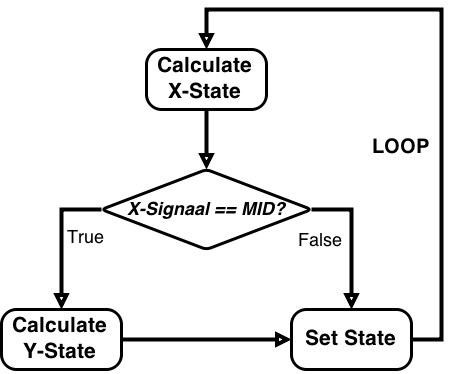
\includegraphics[width=0.7\linewidth]{images/GevoeligheidY}
\caption{Algoritmisch schema voor gevoeligheid van Y-signaal.}
\label{fig:algogevoeligheidY}
\end{figure}

\subsection{Knipperen van het oog}
Om het probleem van oogknipperingen of beter gekend, \textit{blinks }op te lossen, is er eerst de vraag gesteld wat juist de voorwaarden zijn van een blink en hoe deze best kunnen gebruikt worden om blinks te herkennen en weg te filteren uit het signaal. Uit onderzoek \cite{Bulling:eyeanalysis} blijkt dat een blink drie belangrijke kenmerken heeft. 
\begin{enumerate}
	\item Een blink manifesteert zich vooral in een positieve uitwijking in het Y-signaal.
	\item De piekwaarde van deze uitwijking varieert, maar er kan vastgesteld worden dat er een minimumwaarde is. Deze minimumwaarde zal bepalen of de gegeven uitwijking wel degelijk het resultaat is van een blink.
	\item Bij een uitwijking die een blink waarde voorstelt, zal de signaalwaarde voor de uitwijking en de signaalwaarde erna relatief gelijk zijn. Met andere woorden, na een blink zal de signaalwaarde zich altijd herstellen naar de waarde die gemeten werd net voor de blink.
\end{enumerate}






Na het vaststellen van deze drie eigenschappen is er gekozen om te werken met een rij (\textit{queue}) die signaalwaarden van het Y-signaal (\textit{eigenschap 1}) zal opslaan. Een parameter die in dit algoritme belangrijk is, is de maximum lengte van de queue (in dit geval 7). Als de queue 'vol' zit wordt bij het toevoegen van een element, het oudste element steeds verwijderd. Elke iteratie wordt de queue ook geanalyseerd en gekeken of er zich een blink in voordoet. Dit wordt gedaan door eerste de relatieve piekwaarde te berekenen (\textit{eigenschap 2}), dit is het verschil tussen de hoogste signaalwaarde binnen de queue en de referentiewaarde ($\frac{queue[first] + queue[last]}{2}$). Daarna wordt het verschil berekent tussen de eerste (\textit{first}) en laatste (\textit{last}) waarde in de queue (\textit{eigenschap 3}). Als de berekende piekwaarde groter is
dan 200 en het berekende verschil kleiner dan 50 dan herkennen we een blink. Vervolgens zal de blink weggefilterd worden door binnen de queue te interpoleren over de eerste en de laatste waarde. Daarna wordt eventueel ook nog de blinkbuffer opgehoogd. De blinkbuffer maakt het mogelijk om een aantal blinks binnen een bepaalde tijdsspanne te interpreteren als commando (vb: een ‘pen-down’ actie binnen een tekenapplicatie). Een schema van het volledige algoritme is weergegeven in figuur \ref{fig:algoblinkfilter}.

\begin{figure}[H]
	\centering
	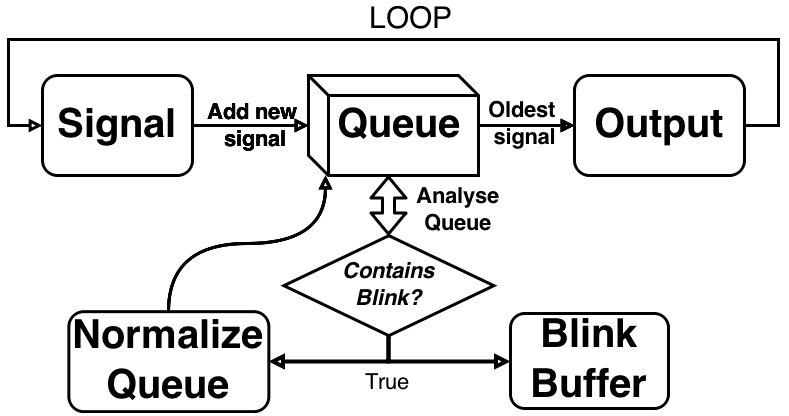
\includegraphics[width = \figwidth]{images/blinkfilterbw}
	\caption{Algoritmisch schema voor het filteren van blinks.}
	\label{fig:algoblinkfilter}
\end{figure}
\subsection{Afdwaling van het signaal}
De afdwaling van het signaal zorgt er voor dat er niet vanuit mag gegaan worden dat de positie van het oog, rechtstreeks in verband staat tot het biopotentiaal. Met andere woorden, er mag dus niet na\"ief aangenomen worden dat er een bepaalde ooghoek overeenkomt met een vast biopotentiaal. Om dit op te lossen wordt er gebruik gemaakt van het verschil in signaal om te bepalen of de toestand is veranderd. Concreet zal het verschil in signaal vergeleken worden met een threshold. Als de waarde hoger ligt dan deze threshold, neemt de applicatie aan dat de toestand veranderd is.\\
\subsubsection*{Toestanden bepalen}
Deze aanpak zorgt tegelijkertijd ook voor een goede manier om de toestand te bepalen. In figuur \ref{fig:algostatefilter} is een schema te zien voor het algoritme dat hiervoor gebruikt wordt.
\begin{figure}[H]
	\centering
	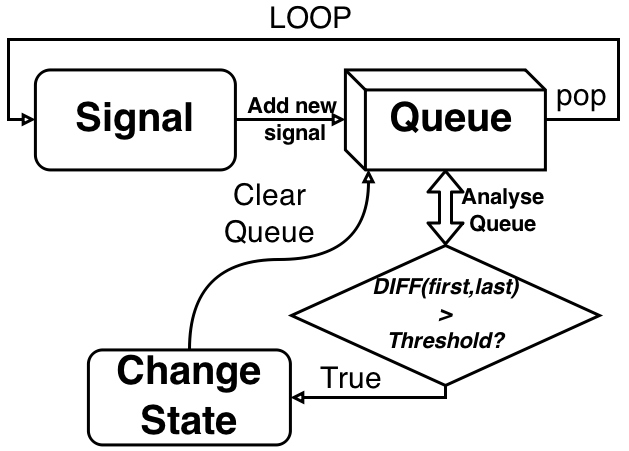
\includegraphics[width=\figwidth]{images/StateFilter_bw}
	\caption{Algoritmisch schema voor het bepalen van toestanden.}
	\label{fig:algostatefilter}
\end{figure}
Een binnenkomend signaal van \'e\'en van de twee richtingen, wordt toegevoegd aan een queue. Daarna zal de queue geanalyseerd worden. Concreet betekent dit dat het verschil tussen het eerste en het laatste element van de queue vergeleken wordt met een threshold. Als deze vergelijking positief uitdraait, wordt de toestand veranderd en de queue geleegd. Dit legen wordt gedaan opdat dezelfde verandering in toestand niet opnieuw wordt geregistreerd.\\
De parameter die bepaalt wat de maximum grootte van de queue is, is afhankelijk van de snelheid van de applicatie. In dit onderzoek is de maximum grootte gelijkgesteld aan 10. De applicatie interpreteert 10 signalen per seconde. Dit betekent dus dat de queue minstens elke seconde nieuwe waarden bevat. Empirisch is vastgesteld dat dit een goede waarde is om het verschil in signaal duidelijk te interpreteren. Deze parameter veranderen heeft rechtstreeks invloed op de gevoeligheid van de applicatie. Als de parameter klein wordt gekozen moet de gebruiker sneller een oogbeweging maken om deze te laten registeren. Bijkomstig is dat de applicatie minder gevoelig is aan trage oogbewegingen. Als de parameter echter groot wordt gekozen, zullen lichtere oogbewegingen makkelijker geregistreerd worden.\\
\subsection{Grenswaarden bepalen}
De grenswaarden (of thresholds) zijn zeer persoonsgebonden. Zelfs de tijd van de dag en de plaatsing van de sensoren hebben een invloed op het biopotentiaal en dus ook op de thresholds. Daarom is het nodig om, voordat de applicatie gestart wordt, de thresholds te bepalen. In de applicatie worden twee thresholds bijgehouden. E\'en voor de X-signalen en \'e\'en voor de Y-signalen. In deze sectie wordt besproken hoe dit probleem in het onderzoek is aangepakt. Daarbovenop wordt er een manier aangeboden om de thresholds te verbeteren doorheen het gebruik van de applicatie.
\subsubsection{Training applicatie}
De training applicatie zal de gebruiker vragen om 10 seconden lang afwisselend in een bepaalde richting  en terug naar het midden te kijken. Dit zal gebeuren voor alle richtingen die geïmplementeerd zijn (in dit geval: links, boven, rechts en onder).
De gehele training zal dus 40 seconden in beslag nemen. Het is de bedoeling om zo voor elk van de richtingen de grootste uitwijkingen te isoleren en hiermee de desbetreffende threshold te berekenen. Gedurende elk van deze periodes van 10 seconden zullen er twee administratieve acties herhaaldelijk uitgevoerd worden:
\begin{enumerate}
	\item Net als bij het algoritme om de toestanden te bepalen, wordt er gebruik gemaakt van een queue waar de corresponderende waardes (afhankelijk van de richting) doorheen schuiven.
	\item Elke keer dat er doorgeschoven wordt, zal de uitwijking binnen de queue berekend worden (verschil tussen eerste en laatste waarde) en de bekomen waarde zal dan opgeslagen worden in een lijst.
\end{enumerate}
Als de 10 seconden verlopen zijn wordt de lijst van verschillen gesorteerd en worden de 50\% kleinste waardes verwijderd uit de lijst, dit wordt gedaan omdat deze waardes waarschijnlijk niet corresponderen met een oogbeweging. Als threshold wordt dan het gemiddelde genomen van de resterende lijst. Aangezien er gebruik gemaakt wordt van \'e\'en threshold per dimensie (verticaal of horizontaal), wordt voor elke dimensie het gemiddelde genomen van de twee corresponderende richtingen 

\subsubsection{Threshold trainer}
De threshold trainer is het mechanisme dat er voor zorgt dat de thresholds doorheen de tijd verbeteren. Eerst wordt het verlagen van de thresholds besproken. Om te voorkomen dat de applicatie geen te lage thresholds aanneemt, wordt er ook een mechanisme om de thresholds te verhogen aangeboden.
\subsubsection*{Verlagen van thresholds}
De eerste thresholdtrainer heeft als doel om de thresholds te verlagen als blijkt dat een oogbeweging niet gedetecteerd is. Maar hoe kan het systeem weten wanneer dit zich voordoet? We kijken even naar volgend scenario:\\

We beginnen in de gebruikelijke beginstand: De gebruiker kijkt naar het midden en het systeem registreert als huidige toestand MIDDEN. Stel dat de gebruiker naar boven kijkt en dus zo tracht om het systeem naar de toestand BOVEN te brengen. Als de verticale threshold te hoog is ingesteld, kan het zijn dat deze beweging dus niet gedetecteerd wordt en het systeem dus nog altijd als huidige toestand MIDDEN aangeeft. Als de gebruiker dan terug naar het midden kijkt om opnieuw te proberen zal er waarschijnlijk een ONDER beweging herkend worden, waardoor de huidige toestand van het systeem DOWN is terwijl de gebruiker gewoon naar het midden kijkt. We zitten dus in een inconsistente toestand, waarbij het systeem denkt dat de gebruiker naar beneden kijkt, terwijl de gebruiker zijn ogen naar het midden heeft gericht. In deze situatie zouden er twee dingen moeten gebeuren:
\begin{itemize}
	\item de huidige toestand van het systeem moet aangepast worden.
	\item De juiste threshold moet aangepast worden (in dit geval de verticale).
\end{itemize}

Het systeem kan niet automatisch weten dat hij een beweging niet herkend heeft, daarom zal de gebruiker opgelegd worden, een actie te ondernemen om dit duidelijk te maken aan het systeem. Om dit te doen is er voor elk van de vier toestanden een nieuwe toestand geïntroduceerd. Voor elke toestand $T$, waarbij $T$ \'e\'en van de vier toestanden voorstelt, is er een extra toestand $T_2$. Deze toestand kan alleen bereikt worden als het systeem als huidige toestand $T$ heeft en er toch nog een extra beweging in deze richting wordt gedetecteerd.  Met andere woorden, het systeem kan alleen in toestand $T_2$ terecht komen als de voorgaande toestand ($T$) incorrect was, want er kan niet naar een richting toe bewogen worden als er in deze richting al gekeken werd. Als het systeem in een van deze nieuwe toestanden komt zal het eerst de huidige toestand aanpassen en daarna de threshold verlagen met 5\%.\\

Als we even terug gaan naar ons vorig scenario dan zien we dat we geëindigd waren in een situatie waar de gebruiker naar het midden keek en het systeem aangaf dat de huidige toestand ONDER was. Met het voorgaande systeem in gedachten zal de gebruiker aangespoord worden om omlaag te kijken om zo de toestand $O_2$ (onder 2) te activeren. Het systeem zal de inconsistente toestand herkennen en de huidige toestand naar ONDER veranderen. Daarbij zal het systeem ook de verticale threshold verlagen, en dit is exact wat er verwacht wordt.\\

Met dit mechanisme wordt er functionaliteit geboden om, met behulp van feedback van de gebruiker, de thresholds te verbeteren. Tegelijkertijd biedt dit mechanisme ook de mogelijkheid om foute interpretatie te melden aan het systeem. Hierdoor kan het systeem zich corrigeren en kan de gebruiker de muisaansturing effici\"ent hervatten.

\subsubsection*{Verhogen van thresholds}\label{sec:verhogenthres}
Als de thresholds verlaagt worden, zal er makkelijker van toestand verandert worden. Om er voor te zorgen dat de threshold dus niet te laag wordt, zal er na elke verandering in toestand, bijgehouden worden welk verschil in signaal deze verandering heeft veroorzaakt. Na een vast aantal waardes verzamelt te hebben wordt het gemiddelde van deze verschillen vergeleken met de huidige threshold. Als het gemiddelde significant hoger ligt dan de huidige threshold, wordt de threshold verhoogt afhankelijk van het gemiddelde. Dit mechanisme is schematisch weergegeven in figuur \ref{fig:algothresholdup}.\\
\begin{figure}[H]
	\centering
	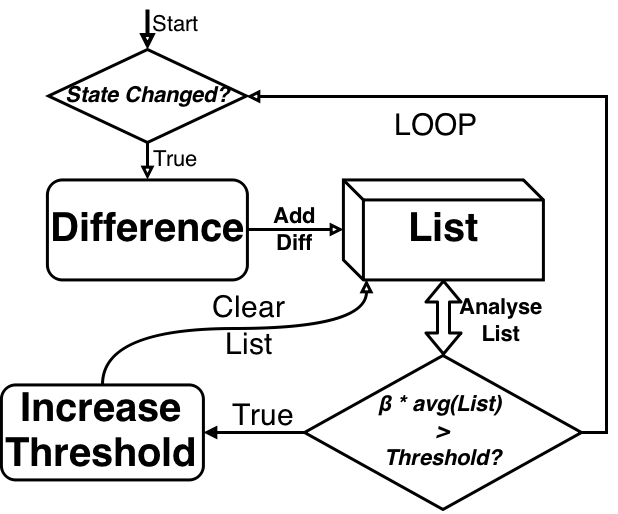
\includegraphics[width=\figwidth]{images/thresholdtrainerup_bw}
	\caption{Algoritmisch schema voor het verhogen van thresholds.}
	\label{fig:algothresholdup}
\end{figure}
Concreet wordt de nieuwe threshold berekent als volgt.
\begin{align*}
	T&: \text{Threshold}\\
	T_a&: \text{Gemiddelde threshold}\\
	\beta \cdot T_a &> T \Rightarrow T = \alpha \cdot T_a
\end{align*}
In dit algoritme duiken opnieuw enkele parameters op die optimaliseerbaar zijn: De grootte van de lijst van verschillen (zie figuur \ref{fig:algothresholdup}) en parameters $\alpha$ en $\beta$. In dit onderzoek zijn deze parameters respectievelijk $5$, $0.8$ en $0.75$. Deze parameters kunnen in verder onderzoek geoptimaliseerd worden.\\ Welke invloed deze parameters hebben op de applicatie zal besproken worden in de experimenten en resultaten.
\section{Experimenten}
Experimenten zijn gedaan op basis van een teken-applicatie. Met de ogen kan de muis aangestuurd worden om te tekenen op het scherm. Met deze functionaliteit is er dan een spel gemaakt dat de gebruiker moet spelen om zo de nauwkeurigheid en de snelheid van het programma te testen. Dit spel bestaat uit het zo snel mogelijk navigeren naar doelen die op het scherm verschijnen. Dit experiment test in eerste instantie de nauwkeurigheid van het programma. Daarnaast is het een goede representatie van de werkelijkheid waarin er met de muis naar knoppen op het scherm zal moeten worden genavigeerd. Er zal een concreet onderscheid gemaakt worden in testen zonder thresholdtraining en met thresholdtraining.\\
\subsection{Geteste waarden}
Er zijn twee referentiewaardes gekozen om de resultaten van de testen te kwantificeren: De genormaliseerde afstand en de genormaliseerde tijd.

\subsubsection*{Genormaliseerde afstand}
Om deze waarde te bekomen wordt eerst de totaal afgelegde afstand berekend, die nodig was om het doel te bereiken (in pixels). Om dit te normaliseren, wordt deze waarde gedeeld door de optimale afstand. Omdat op dit ogenblik, de applicatie geen schuine bewegingen kan maken, is de optimale afstand de \textit{manhatten distance} \cite{manhdist} tussen herkomst en doel. De waarde die wordt bekomen, is hoeveel keer de optimale afstand is afgelegd. Wiskundig kan dit samengevat worden als volgt:
\begin{align*}
	&D_t: \text{Totaal afgelegde afstand}\\
	&D_o: \text{Optimale afstand (manhatten distance)}\\
	&D_n = \frac{D_t}{D_o}
\end{align*}

\subsubsection*{Genormaliseerde tijd}
Om deze waarde te bekomen wordt de tijd, die de gebruiker erover gedaan heeft om een doel te bereiken bepaald. Om dit getal te normaliseren wordt er opnieuw gedeeld door de optimale tijd. De optimale tijd wordt berekend door de optimale afstand te delen door de snelheid van de cursor (In de applicatie 100 pixels/s). De waarde die bekomen wordt, is dan een getal dat zegt hoe veel keer langer er over gedaan is dan de optimale tijd, om het doel te bereiken. Wiskundig kan dit samengevat worden als volgt:
\begin{align*}
	&T_t: \text{Totaal verstreken tijd per doel}\\
	&T_o = \frac{D_o}{v}: \text{Optimale afstand (met } v \text{ het aantal pixels per seconde)}\\
	&T_n = \frac{T_t}{T_o}
\end{align*} 

Deze twee waardes worden gebruikt als resultaat van elke test. Omdat ze genormaliseerd zijn kan er makkelijk gezien worden wanneer een test perfect was (waarde $= 1$) of minder goed (waarde $> 1$).

\subsection{Resultaten}
Met de eerder vermelde experimentopstelling en referentiewaardes ($D_n$ en $T_n$), zijn er concrete resultaten verworven die in deze sectie zullen worden getoond en besproken. Eerst zullen er resultaten zonder thresholdtraining weergegeven worden. Daarna worden de resultaten weergegeven die verworven zijn met dezelfde experimentopstelling maar met de thresholdtrainer. In de experimenten is er steeds gewerkt met sequenties van 80 doelen. Voor elk doel werd er een maximum tijd van 20 seconden toegelaten.
\subsubsection*{Genormaliseerde afstand}

In figuur \ref{fig:resdistnt} wordt de genormaliseerde afstand per bereikt doel weergegeven. Het belangrijkste in deze figuur is de trendlijn (de rechte door de grafiek) die de lineaire regressie van de grafiek voorstelt. Wat meteen opvalt is dat deze trendlijn een rechte is. Concreet wil dit zeggen dat de gemiddelde afgelegde afstand per doel gelijk blijft doorheen het experiment.\\
\begin{figure}[H]
	\centering
	\begin{tikzpicture}
		\begin{axis}[
			width=\figwidth,
			grid=major,
			grid style={dashed,gray!30},
			xlabel=Doelen,
			ylabel=Genormaliseerde afstand,
			ymin = 1,
			ymax = 6
			]
			\addplot +[mark=none] table[x={goals},y={ndist},col sep=semicolon] {data/ndistanceNT.csv};
			\addplot +[mark=none,line width=1pt] table[x={goals},y={create col/linear regression={y=ndist}},col sep=semicolon] {data/ndistanceNT.csv}; 
		\end{axis}
	\end{tikzpicture}
	\caption{Genormaliseerde afstand voor elk doel \textbf{zonder} threshold trainer.}
	\label{fig:resdistnt}
\end{figure}
In figuur \ref{fig:resdistwt} wordt de genormaliseerde afstand per bereikt doel weergegeven, \textbf{met thresholdtrainer}. Meteen is er op te merken dat de trendlijn sterk daalt. Ook zijn er minder uitschieters aanwezig doordat fouten makkelijker gecorrigeerd kunnen worden. De concrete resultaten van de gemiddelde verbetering met en zonder thresholdtrainer zijn weergegeven in tabel \ref{tbl:resgemiddeldesdist}.
\begin{figure}[H]
	\centering
	\begin{tikzpicture}
	\begin{axis}[
	width=\figwidth,
	grid=major,
	grid style={dashed,gray!30},
	xlabel=Doelen,
	ylabel=Genormaliseerde afstand,
	ymin = 1,
	ymax = 6
	]
	\addplot +[mark=none] table[x={goals},y={ndist},col sep=semicolon] {data/ndistanceWT.csv};
	\addplot +[mark=none,line width=1pt] table[x={goals},y={create col/linear regression={y=ndist}},col sep=semicolon] {data/ndistanceWT.csv}; 
	\end{axis}
	\end{tikzpicture}
	\caption{Genormaliseerde afstand voor elk doel \textbf{met} threshold trainer.}
	\label{fig:resdistwt}
	
\end{figure}

\begin{table}[H]
	\begin{tabular}{|c|c|c|}
		\hline  & \textbf{Zonder training} & \textbf{Met training} \\ 
		\hline \textbf{Startgemiddelde} & $1.83$ & $1.79$ \\ 
		\hline \textbf{Eindgemiddelde} & $1.84$ & $1.20$ \\ 
		\hline Verbetering\% & $\mathbf{-0.5}\%$ & $\mathbf{49}\%$\\
		\hline
	\end{tabular} 
	\caption{Resultaten voor gemiddeldes van de genormaliseerde afstand van de experimenten.}
	\label{tbl:resgemiddeldesdist}
\end{table}
Volgens de resultaten in tabel \ref{tbl:resgemiddeldesdist} is er een verbetering van $49$\% tussen het gemiddelde in het begin en het gemiddelde aan het einde van het experiment, als de thresholdtrainer gebruikt wordt.
\subsubsection*{Genormaliseerde tijd}
In figuur \ref{fig:restiment} wordt nu de genormaliseerde tijd voor elk bereikt doel weergegeven, zonder thresholdtrainer. Hetzelfde patroon als bij de genormaliseerde afstand zonder thresholdtrainer, verschijnt: een constante trendlijn.

\begin{figure}[H]
	\centering
	\begin{tikzpicture}
		\begin{axis}[
			width=\figwidth,
			grid=major,
			grid style={dashed,gray!30},
			xlabel=Doelen,
			ylabel=Genormaliseerde tijd,
			ymin = 1,
			ymax = 10
			]
			\addplot +[mark=none] table[x={goals},y={ntime},col sep=semicolon] {data/ntimeNT.csv};
			\addplot +[mark=none,line width=1pt] table[x={goals},y={create col/linear regression={y=ntime}},col sep=semicolon] {data/ntimeNT.csv}; 
		\end{axis}
	\end{tikzpicture}
	\caption{Genormaliseerde tijd voor elk doel \textbf{zonder} threshold trainer.}
	\label{fig:restiment}
	
\end{figure}
Figuur \ref{fig:restimewt} toont de resultaten voor de genormaliseerde tijd \textbf{met} thresholdtrainer. Hier is duidelijk terug een daling van de trendlijn op te merken.

\begin{figure}[H]
	\centering
	\begin{tikzpicture}
	\begin{axis}[
	width=\figwidth,
	grid=major,
	grid style={dashed,gray!30},
	xlabel=Doelen,
	ylabel=Genormaliseerde tijd,
	ymin = 1,
	ymax = 10
	]
	\addplot +[mark=none] table[x={goals},y={ntime},col sep=semicolon] {data/ntimeWT.csv};
	\addplot +[mark=none,line width=1pt] table[x={goals},y={create col/linear regression={y=ntime}},col sep=semicolon] {data/ntimeWT.csv}; 
	\end{axis}
	\end{tikzpicture}
	\caption{Genormaliseerde tijd voor elk doel \textbf{met} threshold trainer.}
	\label{fig:restimewt}
	
\end{figure}

\begin{table}[H]
	\begin{tabular}{|c|c|c|}
		\hline  & \textbf{Zonder training} & \textbf{Met training} \\ 
		\hline \textbf{Startgemiddelde} & $3.76$ & $3.38$ \\ 
		\hline \textbf{Eindgemiddelde} & $3.54$ & $1.86$ \\ 
		\hline Verbetering\% & $\mathbf{6}\%$ & $\mathbf{81.7}\%$\\
		\hline
	\end{tabular} 
	\caption{Resultaten voor gemiddeldes van de genormaliseerde afstand van de experimenten.}
	\label{tbl:resgemiddeldestijd}
\end{table}
De resultaten in tabel \ref{tbl:resgemiddeldestijd} geven nog een beter resultaat dan de genormaliseerde afstand. Dit is vooral te wijten door het feit dat het programma steeds minder fouten maakt en er dus steeds minder tijd wordt verloren. Dit heeft minder invloed op de genormaliseerde afstand, omdat fouten in de interpretatie meestal de beweging stopzetten. Fouten in signaal-interpretatie hebben dus minder invloed op de afgelegde afstand.\\

\subsubsection*{Verandering in thresholds}
In figuur \ref{fig:resthresholds} is te zien hoe de grootte van de thresholds verandert over een lange testprocedure. Het eerste dat opvalt is, dat deze figuur aangeeft dat er heel wat veranderingen worden doorgevoerd. Uit de resultaten van het Y-signaal kan afgeleid worden dat er in deze instantie niet geconvergeerd wordt. Het systeem blijft gedurende het verloop van de test steeds op zoek naar de perfecte thresholdwaarde. Dit geeft aan dat de parameters die gebruikt worden om de thresholds te verhogen (zie sectie \ref{sec:verhogenthres})  eventueel dienen geoptimaliseerd te worden. Ten tweede kan wel vastgesteld worden dat bij het X-signaal er na ongeveer 20 aanpassingen een optimale waarde is gevonden, wat natuurlijk te zien is aan het constante verloop van de grafiek.
\begin{figure}[H]
	\centering
	\begin{tikzpicture}
		\begin{axis}[
			width=\figwidth,
			grid=major,
			grid style={dashed,gray!30},
			xlabel=Correcties,
			ylabel=Thresholdwaarde,
			legend entries={RL-threshold,UD-threshold}
			]
			\addplot +[dashed, mark=none] table[x={alt},y={RL},col sep=semicolon] {data/thresholds.csv};
			\addplot +[scatter, mark=none] table[x={alt},y={UD},col sep=semicolon] {data/thresholds.csv};
			\addplot +[dotted, mark=none] table[x={alt},y={create col/linear regression={y=RL}},col sep=semicolon] {data/thresholds.csv};
			\addplot +[dotted, mark=none] table[x={alt},y={create col/linear regression={y=UD}},col sep=semicolon] {data/thresholds.csv};
		\end{axis}
	\end{tikzpicture}
	\caption{Dynamische correctie van de thresholds.\\\textbf{RL-threshold:} threshold voor horizontale beweging;\\\textbf{UD-threshold:} threshold voor verticale beweging.}
	\label{fig:resthresholds}
\end{figure}

\subsubsection*{Besluit van de resultaten}
Uit de resultaten kan er besloten worden dat de training in het begin van de applicatie voor bruikbare startwaardes zorgt. Verder kan er opgemerkt worden dat het mechanisme om thresholds te trainen, door feedback van de gebruiker, tegelijkertijd een mechanisme aanbiedt om fouten te corrigeren en zo nauwkeuriger en sneller de muisbeweging te controleren. Dit zorgt ervoor dat er een significante verbetering is in de algemene snelheid van de muisaansturing.\\
Tot slot is de algemene verbetering in gemiddelde interpretatie weergegeven in tabel \ref{tbl:resgemiddeldes}. De afstand is voor de experimenten met thresholdtrainer gemiddeld $29\%$ beter. Voor de tijd bedraagt dit een gemiddelde verbetering van $39\%$. In de experimenten was deze verbetering duidelijk zichtbaar en werd de aansturing steeds makkelijker voor de gebruiker.
\begin{table}[H]
	\begin{tabular}{|c||c|c|}
		\hline  & \textbf{Gemiddelde afstand} & \textbf{Gemiddelde tijd} \\ 
		\hline Zonder training & $1.83$ &$3.64$\\ 
		\hline Met training  & $1.42$ & $2.61$\\ 
		\hline verbetering\% & $\mathbf{29\%}$  & $\mathbf{39\%}$ \\ 
		\hline 
	\end{tabular} 
	\caption{Resultaten voor gemiddeldes van de experimenten.}
	\label{tbl:resgemiddeldes}
\end{table}
\section{Conclusie}
Het systeem waar dit onderzoek toe geleid heeft kan duidelijk onderscheid maken tussen de vier rudimentaire bewegingsrichtingen. Door het systeem langer te gebruiken zal het alleen maar beter functioneren in functie van de gebruiker. Eventueel verder onderzoek zou zich kunnen focussen op de verschillende parameters binnen het systeem (queue lengtes, threshold verlagings- en verhogingsfactoren,  etc.) om zo de robuustheid van het systeem te verhogen. In de toekomst zou het ook mogelijk kunnen zijn om volledige tweedimensionale bewegingsvrijheid te implementeren, door bij elke beweging met beide dimensies (X-signaal en Y-signaal) rekening te houden om zo de hoek van de beweging te berekenen.

\nocite{Barea:eogmobility}
\bibliographystyle{named}
\bibliography{EOG}

\end{document}

